\chapter{序論}
\label{c:intro}

近年來,隨著網際網路的快速發展,網際網路中開始出現越來越多彙整人類知識的網站與資源,
如維基百科(Wikipedia)、Freebase等,是透過來自世界各地的志願編輯者一字一句的貢獻建立而成的。

% 為了讓機器可以利用人類的知識來進行一些先進的應用(像是Siri之類的),需要結構化的知識

除了前述網站與資源外,還出現了以其為來源,透過自動化方式產生的結構化資源,
如YAGO、DBpedia等資料庫透過擷取Wikipedia建立結構化的資料庫。


\section{背景介紹}
% Keyword: 知識庫、內容串流

知識庫

如YAGO、DBpedia、Freebase等

內容串流


\section{研究動機}
% Keyword: 知識庫加速
知識庫加速

\section{研究目標}
% Keyword: given a content stream, 回答有沒有某個特性這樣

\section{論文架構}  % TODO FIXME
本論文共分成五個章節。
第一章是緒論,簡介本研究的背景、動機與目標。
第二章是文獻探討,列舉了一些相關的研究與資源。
第三章是研究方法,提出如何於內容串流中究偵測實體特性的方法與步驟。
第四章是實驗結果與分析,
第五章是結論與未來展望,

%\begin{figure}
%\centering
%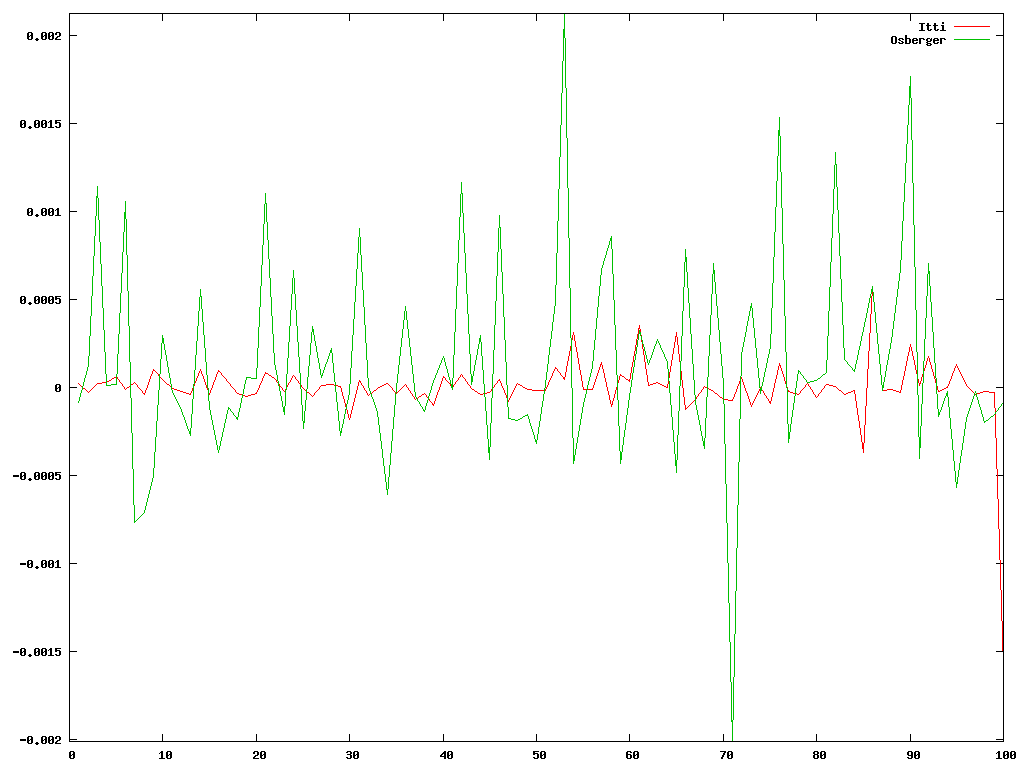
\includegraphics[width=0.45\textwidth]{images/kl}
%\caption{kl-distance}
%\label{kl}
%\end{figure}

%\begin{table}[t]
%\begin{center}
%\begin{tabular}{lcc}
%
%\hline
%                    &  {\small Itti's method}     & {\small Fuzzy growing}    \\
%\hline
%{\small Precision}           &  0.4475    & 0.4506 \\
%{\small Recall}              &  0.5515    & 0.5542 \\
%\hline
%
%\end{tabular}
%\caption[Evaluation of FOA sets]{\small Evaluation of FOA sets. } \label{t:FOA}
%\end{center}
%\end{table}

